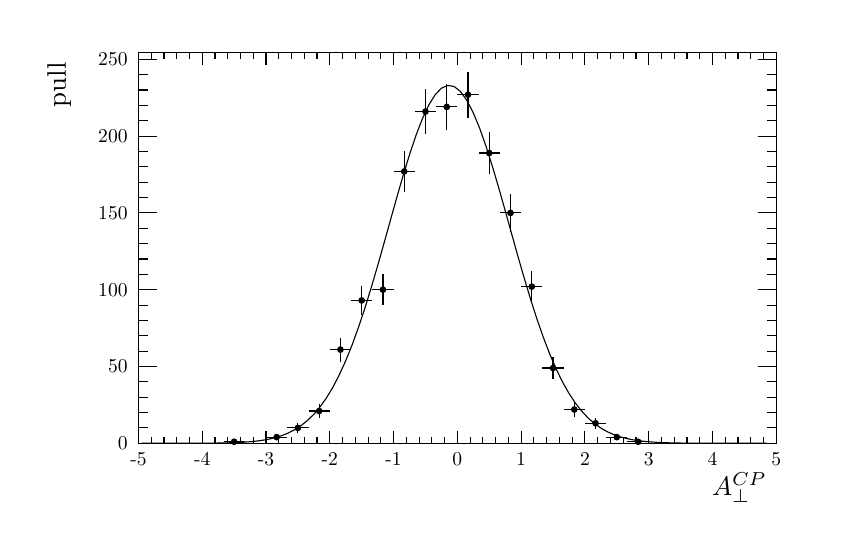
\begin{tikzpicture}
\pgfdeclareplotmark{cross} {
\pgfpathmoveto{\pgfpoint{-0.3\pgfplotmarksize}{\pgfplotmarksize}}
\pgfpathlineto{\pgfpoint{+0.3\pgfplotmarksize}{\pgfplotmarksize}}
\pgfpathlineto{\pgfpoint{+0.3\pgfplotmarksize}{0.3\pgfplotmarksize}}
\pgfpathlineto{\pgfpoint{+1\pgfplotmarksize}{0.3\pgfplotmarksize}}
\pgfpathlineto{\pgfpoint{+1\pgfplotmarksize}{-0.3\pgfplotmarksize}}
\pgfpathlineto{\pgfpoint{+0.3\pgfplotmarksize}{-0.3\pgfplotmarksize}}
\pgfpathlineto{\pgfpoint{+0.3\pgfplotmarksize}{-1.\pgfplotmarksize}}
\pgfpathlineto{\pgfpoint{-0.3\pgfplotmarksize}{-1.\pgfplotmarksize}}
\pgfpathlineto{\pgfpoint{-0.3\pgfplotmarksize}{-0.3\pgfplotmarksize}}
\pgfpathlineto{\pgfpoint{-1.\pgfplotmarksize}{-0.3\pgfplotmarksize}}
\pgfpathlineto{\pgfpoint{-1.\pgfplotmarksize}{0.3\pgfplotmarksize}}
\pgfpathlineto{\pgfpoint{-0.3\pgfplotmarksize}{0.3\pgfplotmarksize}}
\pgfpathclose
\pgfusepathqstroke
}
\pgfdeclareplotmark{cross*} {
\pgfpathmoveto{\pgfpoint{-0.3\pgfplotmarksize}{\pgfplotmarksize}}
\pgfpathlineto{\pgfpoint{+0.3\pgfplotmarksize}{\pgfplotmarksize}}
\pgfpathlineto{\pgfpoint{+0.3\pgfplotmarksize}{0.3\pgfplotmarksize}}
\pgfpathlineto{\pgfpoint{+1\pgfplotmarksize}{0.3\pgfplotmarksize}}
\pgfpathlineto{\pgfpoint{+1\pgfplotmarksize}{-0.3\pgfplotmarksize}}
\pgfpathlineto{\pgfpoint{+0.3\pgfplotmarksize}{-0.3\pgfplotmarksize}}
\pgfpathlineto{\pgfpoint{+0.3\pgfplotmarksize}{-1.\pgfplotmarksize}}
\pgfpathlineto{\pgfpoint{-0.3\pgfplotmarksize}{-1.\pgfplotmarksize}}
\pgfpathlineto{\pgfpoint{-0.3\pgfplotmarksize}{-0.3\pgfplotmarksize}}
\pgfpathlineto{\pgfpoint{-1.\pgfplotmarksize}{-0.3\pgfplotmarksize}}
\pgfpathlineto{\pgfpoint{-1.\pgfplotmarksize}{0.3\pgfplotmarksize}}
\pgfpathlineto{\pgfpoint{-0.3\pgfplotmarksize}{0.3\pgfplotmarksize}}
\pgfpathclose
\pgfusepathqfillstroke
}
\pgfdeclareplotmark{newstar} {
\pgfpathmoveto{\pgfqpoint{0pt}{\pgfplotmarksize}}
\pgfpathlineto{\pgfqpointpolar{44}{0.5\pgfplotmarksize}}
\pgfpathlineto{\pgfqpointpolar{18}{\pgfplotmarksize}}
\pgfpathlineto{\pgfqpointpolar{-20}{0.5\pgfplotmarksize}}
\pgfpathlineto{\pgfqpointpolar{-54}{\pgfplotmarksize}}
\pgfpathlineto{\pgfqpointpolar{-90}{0.5\pgfplotmarksize}}
\pgfpathlineto{\pgfqpointpolar{234}{\pgfplotmarksize}}
\pgfpathlineto{\pgfqpointpolar{198}{0.5\pgfplotmarksize}}
\pgfpathlineto{\pgfqpointpolar{162}{\pgfplotmarksize}}
\pgfpathlineto{\pgfqpointpolar{134}{0.5\pgfplotmarksize}}
\pgfpathclose
\pgfusepathqstroke
}
\pgfdeclareplotmark{newstar*} {
\pgfpathmoveto{\pgfqpoint{0pt}{\pgfplotmarksize}}
\pgfpathlineto{\pgfqpointpolar{44}{0.5\pgfplotmarksize}}
\pgfpathlineto{\pgfqpointpolar{18}{\pgfplotmarksize}}
\pgfpathlineto{\pgfqpointpolar{-20}{0.5\pgfplotmarksize}}
\pgfpathlineto{\pgfqpointpolar{-54}{\pgfplotmarksize}}
\pgfpathlineto{\pgfqpointpolar{-90}{0.5\pgfplotmarksize}}
\pgfpathlineto{\pgfqpointpolar{234}{\pgfplotmarksize}}
\pgfpathlineto{\pgfqpointpolar{198}{0.5\pgfplotmarksize}}
\pgfpathlineto{\pgfqpointpolar{162}{\pgfplotmarksize}}
\pgfpathlineto{\pgfqpointpolar{134}{0.5\pgfplotmarksize}}
\pgfpathclose
\pgfusepathqfillstroke
}
\definecolor{c}{rgb}{1,1,1};
\draw [color=c, fill=c] (0,0) rectangle (10,6.27517);
\draw [color=c, fill=c] (1.4,1.00403) rectangle (9.5,5.96141);
\definecolor{c}{rgb}{0,0,0};
\draw [c] (1.4,1.00403) -- (1.4,5.96141) -- (9.5,5.96141) -- (9.5,1.00403) -- (1.4,1.00403);
\draw [c] (2.615,1.00403) -- (2.615,1.02353);
\draw [c] (2.615,1.02353) -- (2.615,1.04304);
\draw [c] (2.48,1.02353) -- (2.615,1.02353);
\draw [c] (2.615,1.02353) -- (2.75,1.02353);
\foreach \P in {(2.615,1.02353)}{\draw[mark options={color=c,fill=c},mark size=2.402402pt,mark=*,mark size=1pt] plot coordinates {\P};}
\draw [c] (3.155,1.04304) -- (3.155,1.08204);
\draw [c] (3.155,1.08204) -- (3.155,1.12105);
\draw [c] (3.02,1.08204) -- (3.155,1.08204);
\draw [c] (3.155,1.08204) -- (3.29,1.08204);
\foreach \P in {(3.155,1.08204)}{\draw[mark options={color=c,fill=c},mark size=2.402402pt,mark=*,mark size=1pt] plot coordinates {\P};}
\draw [c] (3.425,1.13739) -- (3.425,1.19907);
\draw [c] (3.425,1.19907) -- (3.425,1.26075);
\draw [c] (3.29,1.19907) -- (3.425,1.19907);
\draw [c] (3.425,1.19907) -- (3.56,1.19907);
\foreach \P in {(3.425,1.19907)}{\draw[mark options={color=c,fill=c},mark size=2.402402pt,mark=*,mark size=1pt] plot coordinates {\P};}
\draw [c] (3.695,1.32424) -- (3.695,1.41362);
\draw [c] (3.695,1.41362) -- (3.695,1.50299);
\draw [c] (3.56,1.41362) -- (3.695,1.41362);
\draw [c] (3.695,1.41362) -- (3.83,1.41362);
\foreach \P in {(3.695,1.41362)}{\draw[mark options={color=c,fill=c},mark size=2.402402pt,mark=*,mark size=1pt] plot coordinates {\P};}
\draw [c] (3.965,2.04145) -- (3.965,2.19378);
\draw [c] (3.965,2.19378) -- (3.965,2.34612);
\draw [c] (3.83,2.19378) -- (3.965,2.19378);
\draw [c] (3.965,2.19378) -- (4.1,2.19378);
\foreach \P in {(3.965,2.19378)}{\draw[mark options={color=c,fill=c},mark size=2.402402pt,mark=*,mark size=1pt] plot coordinates {\P};}
\draw [c] (4.235,2.62983) -- (4.235,2.81792);
\draw [c] (4.235,2.81792) -- (4.235,3.00601);
\draw [c] (4.1,2.81792) -- (4.235,2.81792);
\draw [c] (4.235,2.81792) -- (4.37,2.81792);
\foreach \P in {(4.235,2.81792)}{\draw[mark options={color=c,fill=c},mark size=2.402402pt,mark=*,mark size=1pt] plot coordinates {\P};}
\draw [c] (4.505,2.75941) -- (4.505,2.95445);
\draw [c] (4.505,2.95445) -- (4.505,3.14949);
\draw [c] (4.37,2.95445) -- (4.505,2.95445);
\draw [c] (4.505,2.95445) -- (4.64,2.95445);
\foreach \P in {(4.505,2.95445)}{\draw[mark options={color=c,fill=c},mark size=2.402402pt,mark=*,mark size=1pt] plot coordinates {\P};}
\draw [c] (4.775,4.19679) -- (4.775,4.45627);
\draw [c] (4.775,4.45627) -- (4.775,4.71576);
\draw [c] (4.64,4.45627) -- (4.775,4.45627);
\draw [c] (4.775,4.45627) -- (4.91,4.45627);
\foreach \P in {(4.775,4.45627)}{\draw[mark options={color=c,fill=c},mark size=2.402402pt,mark=*,mark size=1pt] plot coordinates {\P};}
\draw [c] (5.045,4.93028) -- (5.045,5.21694);
\draw [c] (5.045,5.21694) -- (5.045,5.50359);
\draw [c] (4.91,5.21694) -- (5.045,5.21694);
\draw [c] (5.045,5.21694) -- (5.18,5.21694);
\foreach \P in {(5.045,5.21694)}{\draw[mark options={color=c,fill=c},mark size=2.402402pt,mark=*,mark size=1pt] plot coordinates {\P};}
\draw [c] (5.315,4.98681) -- (5.315,5.27545);
\draw [c] (5.315,5.27545) -- (5.315,5.56409);
\draw [c] (5.18,5.27545) -- (5.315,5.27545);
\draw [c] (5.315,5.27545) -- (5.45,5.27545);
\foreach \P in {(5.315,5.27545)}{\draw[mark options={color=c,fill=c},mark size=2.402402pt,mark=*,mark size=1pt] plot coordinates {\P};}
\draw [c] (5.585,5.13762) -- (5.585,5.43148);
\draw [c] (5.585,5.43148) -- (5.585,5.72534);
\draw [c] (5.45,5.43148) -- (5.585,5.43148);
\draw [c] (5.585,5.43148) -- (5.72,5.43148);
\foreach \P in {(5.585,5.43148)}{\draw[mark options={color=c,fill=c},mark size=2.402402pt,mark=*,mark size=1pt] plot coordinates {\P};}
\draw [c] (5.855,4.42218) -- (5.855,4.69032);
\draw [c] (5.855,4.69032) -- (5.855,4.95846);
\draw [c] (5.72,4.69032) -- (5.855,4.69032);
\draw [c] (5.855,4.69032) -- (5.99,4.69032);
\foreach \P in {(5.855,4.69032)}{\draw[mark options={color=c,fill=c},mark size=2.402402pt,mark=*,mark size=1pt] plot coordinates {\P};}
\draw [c] (6.125,3.69078) -- (6.125,3.92966);
\draw [c] (6.125,3.92966) -- (6.125,4.16854);
\draw [c] (5.99,3.92966) -- (6.125,3.92966);
\draw [c] (6.125,3.92966) -- (6.26,3.92966);
\foreach \P in {(6.125,3.92966)}{\draw[mark options={color=c,fill=c},mark size=2.402402pt,mark=*,mark size=1pt] plot coordinates {\P};}
\draw [c] (6.395,2.79647) -- (6.395,2.99346);
\draw [c] (6.395,2.99346) -- (6.395,3.19044);
\draw [c] (6.26,2.99346) -- (6.395,2.99346);
\draw [c] (6.395,2.99346) -- (6.53,2.99346);
\foreach \P in {(6.395,2.99346)}{\draw[mark options={color=c,fill=c},mark size=2.402402pt,mark=*,mark size=1pt] plot coordinates {\P};}
\draw [c] (6.665,1.8232) -- (6.665,1.95973);
\draw [c] (6.665,1.95973) -- (6.665,2.09626);
\draw [c] (6.53,1.95973) -- (6.665,1.95973);
\draw [c] (6.665,1.95973) -- (6.8,1.95973);
\foreach \P in {(6.665,1.95973)}{\draw[mark options={color=c,fill=c},mark size=2.402402pt,mark=*,mark size=1pt] plot coordinates {\P};}
\draw [c] (6.935,1.34164) -- (6.935,1.43312);
\draw [c] (6.935,1.43312) -- (6.935,1.5246);
\draw [c] (6.8,1.43312) -- (6.935,1.43312);
\draw [c] (6.935,1.43312) -- (7.07,1.43312);
\foreach \P in {(6.935,1.43312)}{\draw[mark options={color=c,fill=c},mark size=2.402402pt,mark=*,mark size=1pt] plot coordinates {\P};}
\draw [c] (7.205,1.18726) -- (7.205,1.25758);
\draw [c] (7.205,1.25758) -- (7.205,1.32791);
\draw [c] (7.07,1.25758) -- (7.205,1.25758);
\draw [c] (7.205,1.25758) -- (7.34,1.25758);
\foreach \P in {(7.205,1.25758)}{\draw[mark options={color=c,fill=c},mark size=2.402402pt,mark=*,mark size=1pt] plot coordinates {\P};}
\draw [c] (7.475,1.04304) -- (7.475,1.08204);
\draw [c] (7.475,1.08204) -- (7.475,1.12105);
\draw [c] (7.34,1.08204) -- (7.475,1.08204);
\draw [c] (7.475,1.08204) -- (7.61,1.08204);
\foreach \P in {(7.475,1.08204)}{\draw[mark options={color=c,fill=c},mark size=2.402402pt,mark=*,mark size=1pt] plot coordinates {\P};}
\draw [c] (7.745,1.00403) -- (7.745,1.02353);
\draw [c] (7.745,1.02353) -- (7.745,1.04304);
\draw [c] (7.61,1.02353) -- (7.745,1.02353);
\draw [c] (7.745,1.02353) -- (7.88,1.02353);
\foreach \P in {(7.745,1.02353)}{\draw[mark options={color=c,fill=c},mark size=2.402402pt,mark=*,mark size=1pt] plot coordinates {\P};}
\draw [c,line width=0.4] (1.4405,1.00403) -- (1.5215,1.00403) -- (1.6025,1.00403) -- (1.6835,1.00403) -- (1.7645,1.00403) -- (1.8455,1.00403) -- (1.9265,1.00403) -- (2.0075,1.00403) -- (2.0885,1.00457) -- (2.1695,1.00488) -- (2.2505,1.00534) --
 (2.3315,1.00603) -- (2.4125,1.00704) -- (2.4935,1.00852) -- (2.5745,1.01064) -- (2.6555,1.01367) -- (2.7365,1.01792) -- (2.8175,1.02382) -- (2.8985,1.03191) -- (2.9795,1.04287) -- (3.0605,1.05755) -- (3.1415,1.07696) -- (3.2225,1.10229) --
 (3.3035,1.13496) -- (3.3845,1.17655) -- (3.4655,1.22884) -- (3.5465,1.29371) -- (3.6275,1.37316) -- (3.7085,1.46917) -- (3.7895,1.58365) -- (3.8705,1.71829) -- (3.9515,1.87444) -- (4.0325,2.05294) -- (4.1135,2.25401) -- (4.1945,2.47709) --
 (4.2755,2.72072) -- (4.3565,2.98242) -- (4.4375,3.2587) -- (4.5185,3.54504) -- (4.5995,3.83596) -- (4.6805,4.12514) -- (4.7615,4.40565) -- (4.8425,4.67022) -- (4.9235,4.91151) -- (5.0045,5.12243) -- (5.0855,5.29655) -- (5.1665,5.42836) --
 (5.2475,5.51358) -- (5.3285,5.54942) -- (5.4095,5.53468);
\draw [c,line width=0.4] (5.4095,5.53468) -- (5.4905,5.46985) -- (5.5715,5.35708) -- (5.6525,5.20005) -- (5.7335,5.00378) -- (5.8145,4.77436) -- (5.8955,4.51864) -- (5.9765,4.24389) -- (6.0575,3.95746) -- (6.1385,3.66647) -- (6.2195,3.3775) --
 (6.3005,3.0964) -- (6.3815,2.82811) -- (6.4625,2.57657) -- (6.5435,2.34467) -- (6.6245,2.13428) -- (6.7055,1.94632) -- (6.7865,1.7809) -- (6.8675,1.63741) -- (6.9485,1.51469) -- (7.0295,1.41117) -- (7.1105,1.32504) -- (7.1915,1.25432) --
 (7.2725,1.19701) -- (7.3535,1.15117) -- (7.4345,1.11497) -- (7.5155,1.08675) -- (7.5965,1.06503) -- (7.6775,1.04851) -- (7.7585,1.0361) -- (7.8395,1.0269) -- (7.9205,1.02015) -- (8.0015,1.01527) -- (8.0825,1.01178) -- (8.1635,1.00932) --
 (8.2445,1.00759) -- (8.3255,1.0064) -- (8.4065,1.0056) -- (8.4875,1.00505) -- (8.5685,1.00469) -- (8.6495,1.00403) -- (8.7305,1.00403) -- (8.8115,1.00403) -- (8.8925,1.00403) -- (8.9735,1.00403) -- (9.0545,1.00403) -- (9.1355,1.00403) --
 (9.2165,1.00403) -- (9.2975,1.00403) -- (9.3785,1.00403);
\draw [c,line width=0.4] (9.3785,1.00403) -- (9.4595,1.00403);
\draw [c,line width=0.4] (1.4,1.00403) -- (9.5,1.00403);
\draw [anchor= east] (9.5,0.441772) node[scale=0.96888, rotate=0]{$A^{CP}_{\perp}$};
\draw [c,line width=0.4] (1.4,1.15651) -- (1.4,1.00403);
\draw [c,line width=0.4] (1.562,1.08027) -- (1.562,1.00403);
\draw [c,line width=0.4] (1.724,1.08027) -- (1.724,1.00403);
\draw [c,line width=0.4] (1.886,1.08027) -- (1.886,1.00403);
\draw [c,line width=0.4] (2.048,1.08027) -- (2.048,1.00403);
\draw [c,line width=0.4] (2.21,1.15651) -- (2.21,1.00403);
\draw [c,line width=0.4] (2.372,1.08027) -- (2.372,1.00403);
\draw [c,line width=0.4] (2.534,1.08027) -- (2.534,1.00403);
\draw [c,line width=0.4] (2.696,1.08027) -- (2.696,1.00403);
\draw [c,line width=0.4] (2.858,1.08027) -- (2.858,1.00403);
\draw [c,line width=0.4] (3.02,1.15651) -- (3.02,1.00403);
\draw [c,line width=0.4] (3.182,1.08027) -- (3.182,1.00403);
\draw [c,line width=0.4] (3.344,1.08027) -- (3.344,1.00403);
\draw [c,line width=0.4] (3.506,1.08027) -- (3.506,1.00403);
\draw [c,line width=0.4] (3.668,1.08027) -- (3.668,1.00403);
\draw [c,line width=0.4] (3.83,1.15651) -- (3.83,1.00403);
\draw [c,line width=0.4] (3.992,1.08027) -- (3.992,1.00403);
\draw [c,line width=0.4] (4.154,1.08027) -- (4.154,1.00403);
\draw [c,line width=0.4] (4.316,1.08027) -- (4.316,1.00403);
\draw [c,line width=0.4] (4.478,1.08027) -- (4.478,1.00403);
\draw [c,line width=0.4] (4.64,1.15651) -- (4.64,1.00403);
\draw [c,line width=0.4] (4.802,1.08027) -- (4.802,1.00403);
\draw [c,line width=0.4] (4.964,1.08027) -- (4.964,1.00403);
\draw [c,line width=0.4] (5.126,1.08027) -- (5.126,1.00403);
\draw [c,line width=0.4] (5.288,1.08027) -- (5.288,1.00403);
\draw [c,line width=0.4] (5.45,1.15651) -- (5.45,1.00403);
\draw [c,line width=0.4] (5.612,1.08027) -- (5.612,1.00403);
\draw [c,line width=0.4] (5.774,1.08027) -- (5.774,1.00403);
\draw [c,line width=0.4] (5.936,1.08027) -- (5.936,1.00403);
\draw [c,line width=0.4] (6.098,1.08027) -- (6.098,1.00403);
\draw [c,line width=0.4] (6.26,1.15651) -- (6.26,1.00403);
\draw [c,line width=0.4] (6.422,1.08027) -- (6.422,1.00403);
\draw [c,line width=0.4] (6.584,1.08027) -- (6.584,1.00403);
\draw [c,line width=0.4] (6.746,1.08027) -- (6.746,1.00403);
\draw [c,line width=0.4] (6.908,1.08027) -- (6.908,1.00403);
\draw [c,line width=0.4] (7.07,1.15651) -- (7.07,1.00403);
\draw [c,line width=0.4] (7.232,1.08027) -- (7.232,1.00403);
\draw [c,line width=0.4] (7.394,1.08027) -- (7.394,1.00403);
\draw [c,line width=0.4] (7.556,1.08027) -- (7.556,1.00403);
\draw [c,line width=0.4] (7.718,1.08027) -- (7.718,1.00403);
\draw [c,line width=0.4] (7.88,1.15651) -- (7.88,1.00403);
\draw [c,line width=0.4] (8.042,1.08027) -- (8.042,1.00403);
\draw [c,line width=0.4] (8.204,1.08027) -- (8.204,1.00403);
\draw [c,line width=0.4] (8.366,1.08027) -- (8.366,1.00403);
\draw [c,line width=0.4] (8.528,1.08027) -- (8.528,1.00403);
\draw [c,line width=0.4] (8.69,1.15651) -- (8.69,1.00403);
\draw [c,line width=0.4] (8.852,1.08027) -- (8.852,1.00403);
\draw [c,line width=0.4] (9.014,1.08027) -- (9.014,1.00403);
\draw [c,line width=0.4] (9.176,1.08027) -- (9.176,1.00403);
\draw [c,line width=0.4] (9.338,1.08027) -- (9.338,1.00403);
\draw [c,line width=0.4] (9.5,1.15651) -- (9.5,1.00403);
\draw [anchor=base] (1.4,0.721644) node[scale=0.708027, rotate=0]{-5};
\draw [anchor=base] (2.21,0.721644) node[scale=0.708027, rotate=0]{-4};
\draw [anchor=base] (3.02,0.721644) node[scale=0.708027, rotate=0]{-3};
\draw [anchor=base] (3.83,0.721644) node[scale=0.708027, rotate=0]{-2};
\draw [anchor=base] (4.64,0.721644) node[scale=0.708027, rotate=0]{-1};
\draw [anchor=base] (5.45,0.721644) node[scale=0.708027, rotate=0]{0};
\draw [anchor=base] (6.26,0.721644) node[scale=0.708027, rotate=0]{1};
\draw [anchor=base] (7.07,0.721644) node[scale=0.708027, rotate=0]{2};
\draw [anchor=base] (7.88,0.721644) node[scale=0.708027, rotate=0]{3};
\draw [anchor=base] (8.69,0.721644) node[scale=0.708027, rotate=0]{4};
\draw [anchor=base] (9.5,0.721644) node[scale=0.708027, rotate=0]{5};
\draw [c,line width=0.4] (1.4,5.96141) -- (9.5,5.96141);
\draw [c,line width=0.4] (1.4,5.80892) -- (1.4,5.96141);
\draw [c,line width=0.4] (1.562,5.88517) -- (1.562,5.96141);
\draw [c,line width=0.4] (1.724,5.88517) -- (1.724,5.96141);
\draw [c,line width=0.4] (1.886,5.88517) -- (1.886,5.96141);
\draw [c,line width=0.4] (2.048,5.88517) -- (2.048,5.96141);
\draw [c,line width=0.4] (2.21,5.80892) -- (2.21,5.96141);
\draw [c,line width=0.4] (2.372,5.88517) -- (2.372,5.96141);
\draw [c,line width=0.4] (2.534,5.88517) -- (2.534,5.96141);
\draw [c,line width=0.4] (2.696,5.88517) -- (2.696,5.96141);
\draw [c,line width=0.4] (2.858,5.88517) -- (2.858,5.96141);
\draw [c,line width=0.4] (3.02,5.80892) -- (3.02,5.96141);
\draw [c,line width=0.4] (3.182,5.88517) -- (3.182,5.96141);
\draw [c,line width=0.4] (3.344,5.88517) -- (3.344,5.96141);
\draw [c,line width=0.4] (3.506,5.88517) -- (3.506,5.96141);
\draw [c,line width=0.4] (3.668,5.88517) -- (3.668,5.96141);
\draw [c,line width=0.4] (3.83,5.80892) -- (3.83,5.96141);
\draw [c,line width=0.4] (3.992,5.88517) -- (3.992,5.96141);
\draw [c,line width=0.4] (4.154,5.88517) -- (4.154,5.96141);
\draw [c,line width=0.4] (4.316,5.88517) -- (4.316,5.96141);
\draw [c,line width=0.4] (4.478,5.88517) -- (4.478,5.96141);
\draw [c,line width=0.4] (4.64,5.80892) -- (4.64,5.96141);
\draw [c,line width=0.4] (4.802,5.88517) -- (4.802,5.96141);
\draw [c,line width=0.4] (4.964,5.88517) -- (4.964,5.96141);
\draw [c,line width=0.4] (5.126,5.88517) -- (5.126,5.96141);
\draw [c,line width=0.4] (5.288,5.88517) -- (5.288,5.96141);
\draw [c,line width=0.4] (5.45,5.80892) -- (5.45,5.96141);
\draw [c,line width=0.4] (5.612,5.88517) -- (5.612,5.96141);
\draw [c,line width=0.4] (5.774,5.88517) -- (5.774,5.96141);
\draw [c,line width=0.4] (5.936,5.88517) -- (5.936,5.96141);
\draw [c,line width=0.4] (6.098,5.88517) -- (6.098,5.96141);
\draw [c,line width=0.4] (6.26,5.80892) -- (6.26,5.96141);
\draw [c,line width=0.4] (6.422,5.88517) -- (6.422,5.96141);
\draw [c,line width=0.4] (6.584,5.88517) -- (6.584,5.96141);
\draw [c,line width=0.4] (6.746,5.88517) -- (6.746,5.96141);
\draw [c,line width=0.4] (6.908,5.88517) -- (6.908,5.96141);
\draw [c,line width=0.4] (7.07,5.80892) -- (7.07,5.96141);
\draw [c,line width=0.4] (7.232,5.88517) -- (7.232,5.96141);
\draw [c,line width=0.4] (7.394,5.88517) -- (7.394,5.96141);
\draw [c,line width=0.4] (7.556,5.88517) -- (7.556,5.96141);
\draw [c,line width=0.4] (7.718,5.88517) -- (7.718,5.96141);
\draw [c,line width=0.4] (7.88,5.80892) -- (7.88,5.96141);
\draw [c,line width=0.4] (8.042,5.88517) -- (8.042,5.96141);
\draw [c,line width=0.4] (8.204,5.88517) -- (8.204,5.96141);
\draw [c,line width=0.4] (8.366,5.88517) -- (8.366,5.96141);
\draw [c,line width=0.4] (8.528,5.88517) -- (8.528,5.96141);
\draw [c,line width=0.4] (8.69,5.80892) -- (8.69,5.96141);
\draw [c,line width=0.4] (8.852,5.88517) -- (8.852,5.96141);
\draw [c,line width=0.4] (9.014,5.88517) -- (9.014,5.96141);
\draw [c,line width=0.4] (9.176,5.88517) -- (9.176,5.96141);
\draw [c,line width=0.4] (9.338,5.88517) -- (9.338,5.96141);
\draw [c,line width=0.4] (9.5,5.80892) -- (9.5,5.96141);
\draw [c,line width=0.4] (1.4,1.00403) -- (1.4,5.96141);
\draw [anchor= east] (0.392,5.96141) node[scale=0.96888, rotate=90]{pull};
\draw [c,line width=0.4] (1.637,1.00403) -- (1.4,1.00403);
\draw [c,line width=0.4] (1.5185,1.19907) -- (1.4,1.19907);
\draw [c,line width=0.4] (1.5185,1.39411) -- (1.4,1.39411);
\draw [c,line width=0.4] (1.5185,1.58915) -- (1.4,1.58915);
\draw [c,line width=0.4] (1.5185,1.7842) -- (1.4,1.7842);
\draw [c,line width=0.4] (1.637,1.97924) -- (1.4,1.97924);
\draw [c,line width=0.4] (1.5185,2.17428) -- (1.4,2.17428);
\draw [c,line width=0.4] (1.5185,2.36932) -- (1.4,2.36932);
\draw [c,line width=0.4] (1.5185,2.56436) -- (1.4,2.56436);
\draw [c,line width=0.4] (1.5185,2.75941) -- (1.4,2.75941);
\draw [c,line width=0.4] (1.637,2.95445) -- (1.4,2.95445);
\draw [c,line width=0.4] (1.5185,3.14949) -- (1.4,3.14949);
\draw [c,line width=0.4] (1.5185,3.34453) -- (1.4,3.34453);
\draw [c,line width=0.4] (1.5185,3.53957) -- (1.4,3.53957);
\draw [c,line width=0.4] (1.5185,3.73462) -- (1.4,3.73462);
\draw [c,line width=0.4] (1.637,3.92966) -- (1.4,3.92966);
\draw [c,line width=0.4] (1.5185,4.1247) -- (1.4,4.1247);
\draw [c,line width=0.4] (1.5185,4.31974) -- (1.4,4.31974);
\draw [c,line width=0.4] (1.5185,4.51479) -- (1.4,4.51479);
\draw [c,line width=0.4] (1.5185,4.70983) -- (1.4,4.70983);
\draw [c,line width=0.4] (1.637,4.90487) -- (1.4,4.90487);
\draw [c,line width=0.4] (1.5185,5.09991) -- (1.4,5.09991);
\draw [c,line width=0.4] (1.5185,5.29495) -- (1.4,5.29495);
\draw [c,line width=0.4] (1.5185,5.49) -- (1.4,5.49);
\draw [c,line width=0.4] (1.5185,5.68504) -- (1.4,5.68504);
\draw [c,line width=0.4] (1.637,5.88008) -- (1.4,5.88008);
\draw [c,line width=0.4] (1.637,5.88008) -- (1.4,5.88008);
\draw [anchor= east] (1.35,1.00403) node[scale=0.708027, rotate=0]{0};
\draw [anchor= east] (1.35,1.97924) node[scale=0.708027, rotate=0]{50};
\draw [anchor= east] (1.35,2.95445) node[scale=0.708027, rotate=0]{100};
\draw [anchor= east] (1.35,3.92966) node[scale=0.708027, rotate=0]{150};
\draw [anchor= east] (1.35,4.90487) node[scale=0.708027, rotate=0]{200};
\draw [anchor= east] (1.35,5.88008) node[scale=0.708027, rotate=0]{250};
\draw [c,line width=0.4] (9.5,1.00403) -- (9.5,5.96141);
\draw [c,line width=0.4] (9.263,1.00403) -- (9.5,1.00403);
\draw [c,line width=0.4] (9.3815,1.19907) -- (9.5,1.19907);
\draw [c,line width=0.4] (9.3815,1.39411) -- (9.5,1.39411);
\draw [c,line width=0.4] (9.3815,1.58915) -- (9.5,1.58915);
\draw [c,line width=0.4] (9.3815,1.7842) -- (9.5,1.7842);
\draw [c,line width=0.4] (9.263,1.97924) -- (9.5,1.97924);
\draw [c,line width=0.4] (9.3815,2.17428) -- (9.5,2.17428);
\draw [c,line width=0.4] (9.3815,2.36932) -- (9.5,2.36932);
\draw [c,line width=0.4] (9.3815,2.56436) -- (9.5,2.56436);
\draw [c,line width=0.4] (9.3815,2.75941) -- (9.5,2.75941);
\draw [c,line width=0.4] (9.263,2.95445) -- (9.5,2.95445);
\draw [c,line width=0.4] (9.3815,3.14949) -- (9.5,3.14949);
\draw [c,line width=0.4] (9.3815,3.34453) -- (9.5,3.34453);
\draw [c,line width=0.4] (9.3815,3.53957) -- (9.5,3.53957);
\draw [c,line width=0.4] (9.3815,3.73462) -- (9.5,3.73462);
\draw [c,line width=0.4] (9.263,3.92966) -- (9.5,3.92966);
\draw [c,line width=0.4] (9.3815,4.1247) -- (9.5,4.1247);
\draw [c,line width=0.4] (9.3815,4.31974) -- (9.5,4.31974);
\draw [c,line width=0.4] (9.3815,4.51479) -- (9.5,4.51479);
\draw [c,line width=0.4] (9.3815,4.70983) -- (9.5,4.70983);
\draw [c,line width=0.4] (9.263,4.90487) -- (9.5,4.90487);
\draw [c,line width=0.4] (9.3815,5.09991) -- (9.5,5.09991);
\draw [c,line width=0.4] (9.3815,5.29495) -- (9.5,5.29495);
\draw [c,line width=0.4] (9.3815,5.49) -- (9.5,5.49);
\draw [c,line width=0.4] (9.3815,5.68504) -- (9.5,5.68504);
\draw [c,line width=0.4] (9.263,5.88008) -- (9.5,5.88008);
\draw [c,line width=0.4] (9.263,5.88008) -- (9.5,5.88008);
\end{tikzpicture}
